\documentclass[12pt,a4paper]{article}
\usepackage[utf8]{inputenc}

\usepackage{longtable}
\usepackage[utf8]{inputenc}
%\usepackage[T1]{fontenc}
\usepackage{lscape}
%\usepackage{pdfsync}
\usepackage{multirow}
\usepackage{fancyhdr}
\usepackage{graphicx}
\usepackage{lastpage}
\usepackage{afterpage}
\usepackage{lettrine}
\usepackage{color,soul}
\usepackage[dvipsnames]{xcolor}
\usepackage{colortbl}
\usepackage{enumitem}
\usepackage{tikz}
\usepackage{titlesec}





%Palatino font
%\usepackage{pxfonts}
%\usepackage{libertine}
\usepackage[scaled=0.88]{beraserif}
\usepackage[scaled=0.85]{berasans}
\usepackage[scaled=0.84]{beramono}
\usepackage{mathpazo}
%\linespread{1.05}
\usepackage[T1,small,euler-digits]{eulervm}

\usepackage[nomessages]{fp}

\usepackage{amssymb}
\usepackage{amsmath}
\usepackage{siunitx}
\usepackage{bm}



 \definecolor{bleuUCLclair}{rgb}{.09, 0.569, 1}
\definecolor{bleuUCLfonce}{rgb}{ .13, .52, .86}
\definecolor{redBurn}{rgb}{.91, 0.29, 0.08}

\usepackage[colorlinks=true,urlcolor=redBurn,linkcolor=black]{hyperref}
\addtolength{\topmargin}{-1.5cm}
\addtolength{\textheight}{1.5cm}
\addtolength{\textwidth}{2cm}
\addtolength{\footskip}{2cm}
\setlength{\evensidemargin}{-0.5cm}
\setlength{\oddsidemargin}{-0.5cm}
\setlength{\arrayrulewidth}{0.25pt}

\renewcommand{\baselinestretch}{1.1} % Interligne


\newenvironment{maliste}%
{ \begin{list}%
	{\textcolor{bleuUCLfonce}{$\bullet$}\hspace{0.5cm}}%
	{\setlength{\labelwidth}{50pt}%
	 \setlength{\leftmargin}{25pt}%
	 \setlength{\itemsep}{30pt}}}%
{ \end{list} }

%\renewcommand{\headrulewidth}{0.0pt}
%\newcommand{\clearemptydoublepage}{%
%	\newpage{\pagestyle{empty}\cleardoublepage}}




%section like title in longtable
\newcommand{\seclong}[1]{\multicolumn{2}{@{}l}{{\Large\sffamily #1}}
\vspace{0.5cm}
\\}

%enumerate on two columns
\newcounter{listlong}
\newcommand{\newlistlong}{\setcounter{listlong}{1}}
\newcommand{\iteml}[1]{%
\hspace{4.5cm}\textcolor{redBurn}{\arabic{listlong}}\stepcounter{listlong}%
&%
#1%

\\%
}

%left in column
\newcommand{\lcol}[1]{%
\begin{minipage}[t]{.35\textwidth}%

#1%

\end{minipage}%
}

\title{\vspace{-1cm}
\begin{flushleft} {\sffamily Rebuttal for paper \emph{Paper Number} }\end{flushleft}}
\date{\vspace{-1.7cm}\begin{flushleft}\sffamily DeepSphere: Efficient spherical Convolutional Neural Network with HEALPix sampling for cosmological applications, Nathanaël Perraudin, Michaël Defferrard, Tomasz Kacprzak, Raphael Sgier \end{flushleft}}

\pagestyle{fancy}
\fancyhf{}
\fancyfoot[R]{\sffamily\thepage\ / \pageref{LastPage}}
  \fancyfoot[L]{ }

\fancypagestyle{plain}{%
  \fancyhf{}%
  \fancyfoot[R]{\sffamily\thepage\ / \pageref{LastPage}}
  \fancyfoot[L]{ }
}

\renewcommand{\headrulewidth}{0.0pt}


\newcommand{\hlc}[2][yellow]{ {\sethlcolor{#1} \hl{#2}} }

\titleformat{\section}
  {\bfseries\scshape}{Reviewer \# \thesection}{1em}{}

\titleformat{\subsection}
  {\normalfont\scshape}{Comment \# \thesubsection}{1em}{}

\usepackage[framemethod=default]{mdframed}
%\mdfsetup{skipabove=\topskip,skipbelow=\topskip}

\global\mdfdefinestyle{comment}{%
     linecolor=red,linewidth=0.1cm,%
     leftmargin=-0.5cm,rightmargin=-0.5cm, innerleftmargin=0.4cm,innerrightmargin=0.4cm,
     topline=false,bottomline=false
}

\global\mdfdefinestyle{manuscript}{%
     linecolor=gray!20,linewidth=0.05cm,backgroundcolor=gray!20,%
     leftmargin=-0.5cm,rightmargin=-0.5cm, innerleftmargin=0.4cm,innerrightmargin=0.4cm
}

  \renewcommand{\subsectionautorefname}{Comment}

\newcommand{\nati}[1]{{\color[rgb]{.1,.6,.1}{NP: #1}}}
\newcommand{\mdeff}[1]{{\color[rgb]{.1,.6,.1}{MD: #1}}}
\newcommand{\TK}[1]{{\color{red}{TK: #1}}}
\newcommand{\todo}[1]{{\color[rgb]{.6,.1,.6}{TODO: #1}}}



\newcommand{\figref}[1]{Figure~\ref{fig:#1}}
\newcommand{\tabref}[1]{Table~\ref{tab:#1}}
\newcommand{\secref}[1]{Section~\ref{sec:#1}}
%\newcommand{\secref}[1]{\S\ref{sec:#1}}
\newcommand{\eqnref}[1]{(\ref{eqn:#1})}

\renewcommand{\b}[1]{{\bm{#1}}}   % bold symbol

% MATH SYMBOLS
\newcommand{\1}{\b{1}}              % all-ones vector
\newcommand{\0}{\b{0}}              % all-zero vector
\newcommand{\g}[1]{\b{#1}}
\newcommand{\G}{\mathcal{G}}
\newcommand{\V}{\mathcal{V}}
\newcommand{\E}{\mathcal{E}}
\newcommand{\C}{\mathcal{C}}
\newcommand{\B}{\mathcal{B}}
\renewcommand{\L}{\b{L}}
\newcommand{\tL}{\tilde{\L}}
\newcommand{\W}{\b{W}}
\newcommand{\I}{\b{I}}
\newcommand{\D}{\b{D}}
\newcommand{\U}{\b{U}}
\newcommand{\x}{\b{x}}
\newcommand{\X}{\b{X}}
\newcommand{\y}{\b{y}}
\newcommand{\Y}{\b{Y}}
\newcommand{\bu}{\b{u}}
\newcommand{\f}{\b{f}}
\newcommand{\trans}{^\intercal}
\newcommand{\R}{\mathbb{R}}
\newcommand{\bLambda}{\b{\Lambda}}
\newcommand{\blambda}{\b{\lambda}}
\newcommand{\bO}{\mathcal{O}}
\newcommand{\T}{\mathcal{T}}
\DeclareMathOperator*{\esp}{E}
\DeclareMathOperator*{\var}{Var}
\DeclareMathOperator*{\vect}{vec}
\DeclareMathOperator*{\argmin}{arg \, min}
\newcommand{\pkg}[1]{\texttt{#1}}


\begin{document}
\maketitle

% Note: it is very convenient to refer to other comments using the referencing system of \LaTeX, such as here see  \autoref{comment:errorEq2}.

The authors would like to thank the reviewers for their comments, which significantly helped improve the manuscript. We believe we have addressed all the issues raised in the following rebuttal.
%  For each comment, we have first highlighted the issue, then we provided an answer, and finally we described how the manuscript was adjusted.

\section*{Answer to the editor}


\begin{mdframed}[style=comment]
Thank you for submitting your manuscript to Astronomy and Computing. I have received comments from reviewers on your manuscript. Your paper should become acceptable for publication pending suitable minor revision and modification of the article in light of the appended reviewer comments.  In particular, there is a request from a reviewer to have access to the data used in your analysis.

Though this is designated a minor revision, there are quite a few points that need to be addressed before the paper is acceptable for publication.  When resubmitting your manuscript, please carefully consider all issues mentioned in the reviewers' comments, outline every change made point by point, and provide suitable rebuttals for any comments not addressed.
\end{mdframed}

\todo{Answer to editor}

\section{}

\subsection{}

\begin{mdframed}[style=comment]
I have read with great interest the paper by Perraudin and collaborators presenting a methodology (and the associated code) for performing deep machine learning on the sphere using novel algorithms.

The paper is well-written, and the results are clearly presented. The litterature as well as the advantages and limitations of new and existing algorithms are discussed thoroughly and fairly. I recommend this paper for publication, provided the following comments are addressed.
\end{mdframed}

Dear reviewer, we thank you for your time and thorough comments.
The manuscript improved thanks to your feedback.
You'll find an answer to all the points you mentioned in this rebuttal.

\subsection{}
\begin{mdframed}[style=comment]
One fairly significant concern I have is how convincing the application to other machine learning algorithms is. The authors compare deep sphere to a SVM classifier, in the case of distinguising from two cosmological models from density maps. This classification is obviously a simplification of what would be done in real comsological analyses, but is sufficient for the purpose of demonstration here. However, the metrics adopted do not clearly highlight the superiority of DeepSphere. The SVM takes pixel histograms or power spectrum densities (PSDs) of each input map. It is not surprising that DeepSphere outperforms them given that it takes the whole map as input. Histograms and PSDs are very restrictive compressions of the data - dropping a lot of spatial information. An SVM or even a standard fully connected neural network (NN) would perform a lot better. It is unclear how that would compare to DeepSphere. But I would certainly expect DeepSphere to be a lot easier to train and have many fewer parameters, which I think is the key advantage that needs to be highlighted here. This is analogous to comparing a standard convolutional NN to a standard fully-connected NN. With appropriate depth both will extract the same information and perform equally well. But of course the CNN has fewer parameters and is easier to train since its structure naturally extracts spatial information. One wouldn't compare the CNN to a SVM trained on pixel histograms or PSDs, since those would not have access to the same information. It would be more natural to compare the CNN and the NN trained on the same maps, and examine the number of parameters, the time and number of examples needed for training to achieve the same performance, etc. This would truly highlight how the structure of the NN is a key advantage.
\end{mdframed}

We agree that the ML algorithms should be tested on the same input data for a fair comparison.
%In practice, those models are limited by the computational power and the dataset size.

We did try to train an SVM on the raw data but were unable to obtain over $60\%$ accuracy in the three noiseless cases, which is far behind every other tested model.
Practically, the classifier would either overfit or be over-regularized.
We hence decided not to report the raw-data SVM results in the paper.
This information has now been added to the manuscript.
% \nati{FYI, I did try again to be entirely sure about it.}

While fully-connected NNs (FCNNs) generalize CNNs, they don't perform as well as CNNs on tasks where the symmetries exploited by the CNN are relevant.\footnote{For cosmological data on the sphere, a desired symmetry, highlighted in the introduction, is for the model to be invariant to rotations.}
That is similar to our comparison of the FCN and CNN variants.
While the CNN is a generalization, it doesn't perform as well as the FCN.
In practice, the large number of parameters required by a FCNN severely restricts what can be tested on conventional hardware. In our case the input number of pixels (for order $1$) is $1024^2$ which limits the number of neurons that can be used in the architecture. For completeness, we tried a FCNN and were only able to squeeze $128$ neurons in the first layer before hitting an out-of-memory error. With this architecture and a relative amount of noise of $0.5$, we were unable to regularize the network such that it would classify the validation set. (Remember that all reported classifiers obtained close to $100\%$ accuracy in this setting.) Similar conclusions were observed with other settings.
%Furthermore, the harmonic resemblance is another sign that the constructed graph is able to capture the spherical structure of the HEALPix sampling, even when increasing the number of neurons for small part of the sphere (order $2$ and $4$).


\subsection{}
\begin{mdframed}[style=comment]
Page 4: "There is no known point set that achieves the analogue of uniform sampling in Euclidean space and allows exact and invertible discrete spherical harmonic decompositions of arbitrary but band-limited functions." This is ambigious. There exists multiple schemes for performing exact SHT on band-limited signals. Those sampling are more efficient than healpix - often in terms of number of pixels, and sometimes in terms of performance of the spherical harmonic transforms - and more accurate since the transform is exact (at least numerically - so typical errors are machine precision). Healpix transforms are only exact to 1e-7 when using iterative schemes, and that depends on Nside and lmax. Please clarify this paragraph. Obviously healpix is very advantageous for the pooling and other operations that take advantage of its hierarchical nature. This is well discussed in the paper - in particular how the fast graph algorithms could accomodate other sampling schemes.
\end{mdframed}

That is right.
Thanks for pointing it out.
The confusion was due to our ignorance.
We removed the part about exact SHTs from the paragraph as we don't need to make such a point.
%\mdeff{That sentence mostly came from \url{https://healpix.jpl.nasa.gov/html/intronode2.htm}.}
%\mdeff{uniform sampling == same distance between all neighboring pixels}


\subsection{}
\begin{mdframed}[style=comment]
"Our graph is constructed as an approximation of sphere S2, a 2D manifold embedded in R3, Indeed, [33] showed that the graph Laplacian converges to the Laplace-Beltrami when the number of pixels goes to infinity. While our construction will not exactly respect the setting defined by [33], we observe empirically strong evidence of convergence." This paragraph is unclear. Could you please add a few words to clarify what the approach of 33 is?
\end{mdframed}

We tried to clarify the paragraph in the following manner:
\begin{mdframed}[style=manuscript]
Our graph is constructed as an approximation of the sphere $S^2$, a 2D manifold embedded in $\mathbb{R}^3$.
Indeed, \cite{belkin2007convergence} showed that the graph Laplacian converges to the Laplace-Beltrami when the number of pixels goes to infinity providing uniform sampling of the manifold and a fully connected graph built with exponentially decaying weights.
While our construction does not exactly respect their setting (the sampling is not uniform and the graph is not fully connected), we empirically observe a strong correspondence between the eigenmodes of both Laplacians (see Appendix A).
\end{mdframed}

While this particular point deserves more details, we believe that a deeper discussion does not belong to this paper.
In fact, we are currently investigating this convergence with the goal of constructing better graphs whose Fourier modes would converge to (or even be equivalent to) the spherical harmonics.

\subsection{}

\begin{mdframed}[style=comment]
Figure 3: What was resolution used for those maps? Does the projection of the eigenvectors depend on the resolution and band-limit?
\end{mdframed}

Those maps have been produced with a resolution of $N_{side}=16$. The information has been added to the paper. (High resolution is costly as diagonalizing the Laplacian matrix scales as $O(N_{pix}^3)$.)

Since we do not have any convergence result yet, we are not sure about how the projection error evolves. However, if there is convergence (and we believe there is), the eigenvectors associated with the lowest $\ell$ probably converge first.

\subsection{}
\begin{mdframed}[style=comment]
Page 7: "That is much more efficient than filtering with spherical harmonics, even though HEALPix was de- signed as an iso-latitude sampling that has a fast spherical transform. That is especially true for smooth kernels which require a low polynomial degree K. Figure 4 compares the speed of low-pass filtering for Gaussian smoothing using the spherical harmonics and the graph-based method presented here. A naive implementation of our method is ten to twenty times faster for Nside = 2048, with K = 20 and K = 5, respectively, than using the spherical harmonic transform at lmax = 3Nside implemented by the highly optimized libsharp [38] library used by HEALPix." This is not so clear. Is the graph method also performing a Gaussian smoothing with the same characteristics? If so, what are those? How precise is the graph convolution approximating the true harmonic-space Gaussian convolution in this case? This is relevant since some approximations (for instance when analyzing cosmic microwave background data) require high-precision Gaussian smoothing. Finally, is lipsharp optimizing Gaussian smoothing in any way?
\end{mdframed}

The experiment whose result is reported in Figure 4 is intended to report filtering speed, independently of the chosen filter (we used a Gaussian for convenience).
While libsharp is probably not optimizing Gaussian smoothing in particular (w.r.t. filtering with any other filter), it is a highly optimized library for SHT.
We don't care about the approximation quality as, in the context of neural networks, filters are learned.
That is, graph filters are not approximating any predefined true harmonic-space filters anyway.
It is however true that replacing spherical filtering (using the SHT) with graph filtering is an interesting prospect (in terms of speed) that might be possible in the future as suggested by Appendix B (Figure B.13).
We feel that, in its current state, graph filtering is probably not a good enough approximation to be usable when high-precision filtering is required.
Nevertheless, theoretical improvements on a potential equivalence (or convergence) of the Laplacian eigenvectors to the spherical harmonics (see our answer to comment 1.4) could potentially make it competitive.


\section{}

\begin{mdframed}[style=comment]
First of all, I would like to thank the authors for writing such a well thought out paper on such an interesting method.

The paper contains an extremely well described technique for performing convolutions on the sphere by first transforming the sphere into pixel space using graphs and then using graph-based convolutional filters that are radially symmetric. These convolutions are then used in neural networks, with an example showing classification of different cosmological scenarios directly from convergence maps. There are several benefits to this method over previously described neural networks on spheres (such as using spherical harmonics, which is slow, or using 2D CNNs, which has to learn to deal with distortions from the projection). I found the approximation of the graph approaching spherical harmonics extremely fascinating and will certainly looking more into this myself in the future!

I will happily recommend this paper for publication. Firstly though, I would like access to the data (privately rather than via emailing the group) so that I can check the notebooks thoroughly. The notebooks are extremely well written but I would like to run them first. As well as this I think there are a few extra applications which will improve the manuscript further, and make the method more appealing for users. I would recommend that these ideas are at least seriously considered by the authors and hopefully implemented:
\end{mdframed}

\todo{@Tomek: give him access to data}

Dear reviewer, we would like to thank you back for your time, your good words, and your thorough review.
The manuscript substantially improved thanks to your work.
You'll find an answer to all the points you mentioned in this rebuttal.

\subsection{}

\begin{mdframed}[style=comment]
The first, and most important is an example using masks. Since the authors mention how their method should in principle work well with masks, especially in comparison to HEALPix and Clebsh-Gordan transform spherical harmonic methods I think that it would be extremely enlightening to present this work, probably in the form of a performance vs. time plot. With this being done, the informational content of a masked version of the cosmological application could easily be included. This would, I'm sure, be attractive to the cosmological community as well as the ML community who are always looking for good ways to deal with masked data.
\end{mdframed}

We agree with the reviewer that an example with an irregular mask is the most missed.
A performance versus time plot would indeed be a great way to present such a comparison.
As the reviewer hints at, this example would be better presented in the light of a comparison to other formulations of spherical CNNs.
While such a comparison would without any doubt be insightful on many aspects (not only for masked data, but also on the role of isotropic filters or the importance of rotation equivariance), it is better carried out on diverse datasets and tasks, and deserves, in our opinion, a follow-up paper to be properly addressed.
The point of this paper was (1) to show that spherical CNNs are a great model for cosmological applications, and (2) that a graph-based spherical CNN has certain undeniable advantages.
As hinted in the conclusion, we are actively working on a more thorough comparison of graph-based and SHT-based spherical CNNs.

On the practical side, a proper comparison requires to either modify the available implementations of \cite{cohen2018sphericalcnn,esteves2017sphericalcnn,kondor2018clebsch} to use the HEALPix sampling, or to transform the cosmological maps to the sampling schemes they support.
Moreover, implementing the pooling operation for irregular masks is not trivial.
All in all, that is a tremendous amount of engineering work that we preferred to defer.

Keep in mind that, while they are not irregular masks, we already use $1/12$, $1/48$, and $1/192$ parts of the sphere for training and inference.
While an SHT-based method needs to consider the whole sphere to work with this data, our graph-based method only considers the used part (and still takes the curvature of the surface into account).
The computational advantage of doing so has been added to Figure 4.
As stated above, the performance comparison will however have to wait our follow-up work.
% Our main motivation was to build a "large" dataset with a relatively low number of cosmological maps.

% In terms of neural network, the available implementation of \cite{cohen2018sphericalcnn,kondor2018clebsch} for spherical CNNs and Clebsh-Gordan CNNs are not scalable enough to be trained on the cosmological maps dataset and do not use the HEALPix sampling. Hence a comparison with these methods requires a different setting, which far beyond the scope of our contribution.

%\nati{We could compare the price of one convolution. What do you think? We can write the theoretical complexity. This is a sensitive point!}

\mdeff{measure the computational time of filtering on a 1/12, 1/48 or 1/192 of the sphere with the graph. Add the result to Figure 4 and compare with filtering of the full sphere (with SHT and graph).}

\subsection{}

\begin{mdframed}[style=comment]
Secondly, using only SVM as a comparison might skew how well this technique appears to works in a deep learning setting. In principle (and I say this not knowing for sure) 2D CNNs should probably be able to work as well as DeepSphere (although no where near as elegantly) by taking in a projected 2D image of the sky and using *loads* of filters to learn about the distortion at different parts of the projected sky. It would be interesting (and I think a fairly easy test) to check how well DeepSphere performs against a 2D CNN on projections.
\end{mdframed}
\todo{Assigned: @Nati, @Michael, @Tomek}

\nati{\textbf{Very important point!!!}
\begin{itemize}
  \item We can do this comparison...
  \item Since we used 1/12 of the sphere, all the pixel grids we use are somehow squared. I am now using this as a projection. @Tomek, do you know if this is ok? Or do you know how to do the projection in a simple and efficient manner?
  \item I think that traditional 2D CNNs will be as good as our algorithm. We should be very careful in the way we formulate this in our answer and in the paper.
\end{itemize}
}

\begin{mdframed}[style=comment]
Similarly, I think it would useful to check how well the DeepSphere CNN does against the FCN when the input data is rotated randomly during training - I imagine that the results should match or probably exceed the FCN results and I think this would be a neat little test which doesn't involve needing extra data, just more augmentation.
\end{mdframed}
\todo{Assigned: @Nati, @Michael, @Tomek}

Theoretically, providing that the FCN and the CNN have the same modelisation power (i.e, the FCN does not have more or larger layers) and assuming the convolution would be truly invariant to rotation, the CNN could never exceed the FCN for truly rotational invariant data. However, assuming enough augmentation (as suggested by the reviewer) and training, the CNN should get to the level of the FCN. In practice, this would require more training as the CNN has to learn the invariance.
The point of defining a FCN instead of a CNN is to avoid the complexity of augmenting the dataset. Hence we did not implement it. Nevertheless, it is an interesting point worth discussion in the paper. We updated the manuscript accordingly.
\todo{Do it}

\nati{
Technically, testing this is complicated as rotation on HEALPix are complicated and expensive. We probably will have to break a lot of code to do it.

@Michael: what do you think?
}

\subsection*{Minor comment}

\begin{mdframed}[style=comment]
I should say, even though I made the above comments, I thought the paper was really excellent and well written. There were a couple of very minor points which I would like the authors to expand slightly on or consider.
\end{mdframed}
Thank you very much for your comments. We addressed them to the best we could.

\subsection{}
\begin{mdframed}[style=comment]
While our construction will not exactly respect the setting defined by [33], we observe empirically strong evidence of convergence.

- Could you add a plot comparing the graph Laplacian as a function of number of pixels and the Laplace-Beltrami operator so the reader can explicitly see the convergence?
\end{mdframed}

This is a good question and a fair request. Problematically, we cannot provide such a plot without solving the theoretical problem first. Indeed to experimentally show convergence, we actually need to build a series of graph Laplacian that converges toward the Laplace Beltrami operator. This far more complicated than building one Laplacian and observe some similarities between the two operators.

This is actually a problem we are currently investigating. We plan to make a separate contribution.


\subsection{}

\begin{mdframed}[style=comment]
We found out that the one proposed above works well for our purpose, and did not investigate other approaches, leaving it to future work.

- Are you really going to search through different weighting schemes in future work? I would be interested if you were, but could you speculate on what you expect to achieve by looking at different ones?
\end{mdframed}

Yes, we are investigating the question of graph weights.
As suggested in the previous comment, the weighting scheme used is very important for the graph Laplacian to approach the true Laplace Beltrami operator. Using a more appropriate weighting scheme, one could hope for a more rotational invariant convolution and a faster convergence rate of the operator.
\nati{@michael, how much shall we say here?}

\subsection{}
\begin{mdframed}[style=comment]
Thanks to the softmax, the output $\bf{y}\in\mathbb{R}^{N_{classes}}$ of a neural network is a probability distribution over the classes, i.e., $y_i$ is the probability that the input sample belongs to class $i$.

- This is a common misconception which is incorrect and needs restating. It is *not* a probability distribution for the class, rather it is a discretised conditional distribution for the class given both the data and the weights and biases of the trained network. One way to see that the value of $y_i$ cannot be considered a probability (which implies P(y|x), i.e. the probability of a class given the data) is that if the network is untrained, would you retrieve back the correct probability? It's wholly dependent on the network.
\end{mdframed}

We agree with the reviewer. We actually misformulate this sentence. We have reformulated it as:
\begin{mdframed}[style=manuscript]
Thanks to the softmax, the output $\y \in \R^{N_{classes}}$ of a neural network is a probability distribution over the classes, i.e., $y_i$ is the confidence of the network that the input sample belongs to class $i$. Note that in general, this probability distribution does not correspond to the true posterior distribution $p(y|x)$.
\end{mdframed}

\nati{By the way, this mean that the reviewer is knowledgable with ML, and may be Bayesian. He might be working on another spherical approach.}

\subsection{}
\begin{mdframed}[style=comment]
For example, on images, the subject of interest is most often around the center of the picture. (Also... Contrast that with images, where the subject of interest is most often around the center of the picture.)

- I don't see that this is general at all, only if you are considering say, preprocessed postage stamps of galaxies. I can't think of many other cases in modern machine learning where the images contain the informative part only in the centre of an image. I do agree that the informative part is often localised though. Maybe this should be updated.
\end{mdframed}
\todo{Assigned: @michael}

\subsection{}
\begin{mdframed}[style=comment]
Than can be seen as intrinsic data augmentation, as a CNN would need to see many rotated versions of the same data to learn the invariance.

- I think you mean "This" rather than "Than". I think, however, you are making a more important point here than you realise. It is not really "intrinsic data augmentation" but rather building a NN to suit your purposes. This should be done by the entire community as, at the moment, too many people blindly build their networks without considering their data and then struggle to get the best results out. The symmetries of the data should be the first thing to influence architecture of a network, exactly as you have reasoned. You might want to add a statement about how you know what your symmetries are and thus, you know how to build a well reasoned network which is more likely to work (and that other should do the same).
\end{mdframed}
\todo{Assigned: @michael}

\subsection{}
\begin{mdframed}[style=comment]
As such, the SHT is only performed once on the input (no back and forth SHT between each layer). While this clever trick lowers the complexity of the convolution to $\mathcal{O}(N_{pix})$, the non-linearity is $\mathcal{O}(N^{3/2}_{pix})$.

- I don't understand what the difference is between the convolution and the "non-linearity". I think this sentence either needs explaining further. Is the process $\mathcal{O}(N_{pix})$ or $\mathcal{O}(N^{3/2}_{pix})$?
\end{mdframed}
In the work of \cite{kondor2018clebsch}, the convolution is performed in the spectral (harmonic) domain with a simple Adamar product. Instead of recomposing the signal and applying a traditional non-linearity such as "relu" in the pixel domain, \cite{kondor2018clebsch} proposes to directly apply a Clebsch–Gordan product in the spectral domain. As a non-linear operation preserving the rotation equivariance, it is considered as the non-linearity of the neural network.

We have modified the manuscript as:
\begin{mdframed}[style=manuscript]
While this clever trick lowers the complexity of the convolution (Adamar product in the spectral domain) to $\bO(N_{pix})$, the non-linearity (Clebsch–Gordan product) is $\bO(N_{pix}^{3/2})$.
\end{mdframed}
\nati{Should we be clearer in the paper?}

\subsection{}
\begin{mdframed}[style=comment]
When mentioning that you are 10 to 20 times faster than the SHT it should be noted that libsharp has amazing distributed mpi functionality which helps, although of course your method is genuinely lower order computationally (and can be distributed simply on a GPU).
\end{mdframed}
When comparing the speed, we used a single-core CPU implementation of the graph convolution. We believe that this comparison is fair.
\nati{Is this sufficient?}

\subsection{}
\begin{mdframed}[style=comment]
In Appendix A. (my personal favourite part) could you measure the percent difference that different eigenvectors differ from the spherical harmonics due to incomplete discretisation of the sphere, perhaps plotting side by side plots like Figure 3, but with SH too (or their differences). By the way, Figure A.12 is placed in the wrong section.
\end{mdframed}
\todo{Assigned: @nati, @michael}
We added a figure showing the percentage of mis-alignment with the spherical harmonics. We also moved Figure A.12 in the correct subsection.

\begin{center}
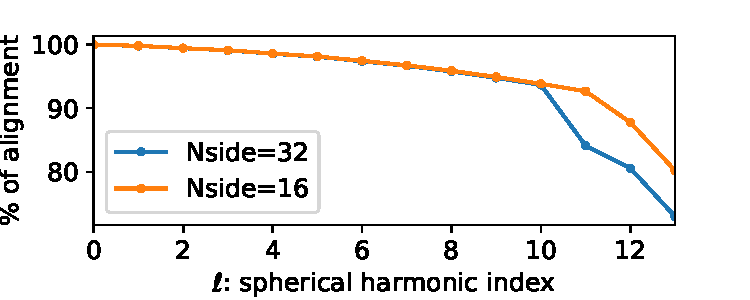
\includegraphics[width=0.5\linewidth]{figures/subspace_alignment_percentage.pdf}
\end{center}

\subsection{}
\begin{mdframed}[style=comment]
In Appendix C. is there a connection between $t$ and $\sigma$ that you can make, or do you just fit them to be similar? If you just fit them to be similar I'm not sure where the relative differences come from. If they are related, however, then the relative differences make sense, but I can't see what the connection is.
\end{mdframed}

In the current version of the manuscript and the code, we simply fitted a few $t$ to match the different $\sigma$. In theory, there should be a connection between the two values providing the graph Laplacian has converged toward the Laplace Beltrami operator. Again, this is left for a futur contribution.

\subsection{}
\begin{mdframed}[style=comment]
A question that I would like to know personally, are you thinking about a future upgrade to non-radial kernels?
\end{mdframed}
We are thinking about it. However, as the graph framework we are using only works with radial filters, it is not a simple question. One simple trick to make the network sensitive to direction is to add a per-channel fully connected layers. We are currently investigating other potential graph techniques that would lead to non-radial kernels.


\subsection{Details}
\begin{mdframed}[style=comment]
Finally, I noticed a few points in the text where there were typos or things which were difficult to follow and I have put a note of them below and tried to correct them as much as I can so that you don't have to put too much effort in - I can't wait to see this paper published. Sorry that the list is so extensive (I'm a bit of a stickler for details and trying to write papers concisely):
\end{mdframed}
\todo{Assigned @tomek.
This reviewer really spend the time. Should we say something here?}

\begin{mdframed}[style=comment]
Convolutional Neural Networks (CNNs) have been proposed as an alternative analysis tool in cosmology thanks to their ability to automatically design relevant statistics to maximise the precision of the parameter estimation [9–16].

- There are many of us in the community who are not overly keen on "precision" of parameter estimation being the target for machine learning. Rather, we would prefer robustness of parameter estimation. It might be worth changing this sentence a bit so as not to upset some of the referenced authors ;)
\end{mdframed}
\todo{Assigned: @tomek, @michael}

\begin{mdframed}[style=comment]
When you have multiple = in equations could you split them on to separate lines? This would make the logical steps for following the equations a lot clearer.
\end{mdframed}
\todo{Assigned: @tomek}
\nati{I personally think it is better without separating the lines}

\begin{mdframed}[style=comment]
You change a lot between "node", "vertex" and "pixel". Could you stick to one of these? I think that "vertex" or "pixel" makes the most sense ("pixel" due to the HEALPix pixelisation of the maps or vertex because of the use of the $v$ notation). Node is quite confusing in several places because there is an inherent connection between node and neuron in ML literature, and since there is swapping between the three different terms it's a little hard to keep track.
\end{mdframed}
\todo{Assigned: @all}
\nati{What do you think? This avoid repetition. But we could be more consistent...}


\begin{mdframed}[style=comment]
You change between math font and text font for the names of your layers when inside and outside of equations. It would look a lot neater sticking with one choice. (Sorry, that seems quite petty and I don't mean it to be).
\end{mdframed}
Thank you for the suggestion. We have made the paper consistent.
\nati{@all, when you read the paper, please check that I did not forget some of them. Every layer has been changed to math symbols as we use them like function. For example, SM becomes $SM$.}

\begin{mdframed}[style=comment]
In Appendix C. you talk about Kroneker a lot, but earlier you talk about Kroneker $\delta$ (which is it's correct name). It's probably worth sticking with the full name.
\end{mdframed}
We have modified the manuscript according to the reviewer suggestion.

\begin{mdframed}[style=comment]
Sky maps are rotation invariant: rotating maps on the sphere doesn’t change their interpretation, as only the statistics of the maps are relevant.
- I think that you mean that rotating maps on the sphere doesn't change their interpretation *when* only the statistics of the maps are relevant. Say you wanted to compare the NGC against the SGC, then rotating the map would obviously change the results.
\end{mdframed}
This sentence has been reformulated as:
\begin{mdframed}[style=manuscript]
We consider the sky maps rotational invariant as in our case rotating maps on the sphere doesn't change their interpretation since only the statistics of the maps are relevant.
\end{mdframed}

\begin{mdframed}[style=comment]
The flexibility of modelling the data domain with a graph allows to easily model data that spans only a part of the sphere, or data that is not uniformly sampled.

- I think you're missing a "one" after allows. "The flexibility of modelling the data domain with a graph allows one to easily model data that spans only a part of the sphere, or data that is not uniformly sampled."
\end{mdframed}
\todo{assigned: @tomek}
\nati{I am not sure of the english here.}

\begin{mdframed}[style=comment]
This kind of maps can be created using the gravitational lensing technique [see 29, for review]

- It should be "These" and not "This". "These kind of maps can be created using the gravitational lensing technique [see 29, for review]"
\end{mdframed}
Thank you for spotting this mistake. We updated the manuscript.

\begin{mdframed}[style=comment]
A CNN is composed of the following main building blocks [31]: (i) a convolution, (ii) a non-linearity, (iii) a down-sampling operation, (iv) a pooling operation, and (v), optionally, normalization.

- I think that this is generalising a CNN a bit too much. In my mind (and in my personal uses of CNNs) steps (iii) and (iv) are not always necessary either. Perhaps you want to say that you wish to tackle common tasks which often arise in CNNs: i) convolution, (ii) non-linearity, (iii) down-sampling operation, (iv) pooling operation, and (v), optionally, normalisation.
\end{mdframed}
\todo{assigned: @michael}


\begin{mdframed}[style=comment]
Likewise, down-sampling can be achieved by taking one pixel out of n.

- I'm afraid I don't understand what this means at all, could you rephrase it?
\end{mdframed}
This has been rephrased as:
\begin{mdframed}[style=manuscript]
Likewise, down-sampling can be achieved by keeping one pixel every $n$ pixels with $n=2$ being very common.
\end{mdframed}

\begin{mdframed}[style=comment]
A rhombus is a quadrilateral whose four sides all have the same length.

- I'm not sure that this really needs to be said.
\end{mdframed}
\todo{assigned: @michael}

\begin{mdframed}[style=comment]
As each pixel is subdivided in four, the second coarser resolution is $N_{pix} = N_{side}^2\times12=2^2\times12=48$ pixels (middle sphere in Figure 5), the third is $N_{pix} = N_{side}^2\times12=42\times12=192$ pixels, etc., where $N_side =1,2,4,8,\dots$ is the grid resolution parameter.

- Might it be more concise to write "The resolution changes as $N_{pix} = N^2_{side}\times12$ such that $N_{pix} = 48$ for $N_{side} = 2$ and $N_{pix} = 192$ with $N_{side}=3$."
\end{mdframed}
\todo{assigned: @tomek}

\begin{mdframed}[style=comment]
... is a measure of the variation of the eigenvector $\bf{u}_i$ is on the graph defined by the Laplacian L.

 - I don't think the "is" after $\bf{u}_i$ should be there.
\end{mdframed}
This has been corrected.

\begin{mdframed}[style=comment]
Given the convolution kernel $h:\mathbb{R}_+ \to \mathbb{R}$,a signal $f\in\mathbb{R}^{N_{pix}}$ on the graph is filtered as

- You don't mention what $\mathbb{R}_+$ is or why $h$ defines that map.
\end{mdframed}
\nati{This seems clear to me. Specifying what $\mathbb{R}_+$ is would be a bit too much I believe. @all -> is it also for you?}

\begin{mdframed}[style=comment]
This localization of the kernel $h$ can be useful to visualize kernels, as explained in Appendix C.

 - Most of Appendix C is not involved with the localisation of the kernel so it might be worth expanding this sentence to "This localisation of the kernel $h$ can be useful to visualise kernels, as shown in an example of heat diffusion presented Appendix C. " Also, it is a little odd that Appendix C is mentioned before Appendix B in the text.
\end{mdframed}
We followed both of the reviewer suggestions.

\begin{mdframed}[style=comment]
However, when considering only parts of the sphere, one can observe important border effects (see Figure B.13 and Appendix B).

- I would just refer the reader to the appendix rather than the figure and the appendix. It is a bit more concise. "However, when considering only parts of the sphere, one can observe important border effects (see Appendix B)."
\end{mdframed}
We changed the manuscript according to the reviewer suggestion.

\begin{mdframed}[style=comment]
... where $T_ig[j]=g[i-j]$ is, up to a flip, a translation operator.

 - I don't understand what you mean by a "flip", a change of sign, the inversion of the kernel?
\end{mdframed}

We updated the manuscript using:
\begin{mdframed}[style=manuscript]
where $T_i g[j] = g[i-j]$ is, up to a flip ($g[i-j]$ instead of $g[i+j]$), a translation operator.
\end{mdframed}

\begin{mdframed}[style=comment]
Similarly as (2), the convolution of the signal $f$ by a kernel $g$ is the scalar product of $f$ with translated versions $T_ig$ of the kernel $g$.

- I think this should be "As with equation (2)" or "Similarly, as in equation (2)" but I can't tell which. Also, it would be really useful if you referred to equations by "equation (x)" rather than just "(x)" throughout - much easier to read that way.
\end{mdframed}
\todo{Assign: @michael, @tomek}
\nati{I do not know what we should do.}

\begin{mdframed}[style=comment]
The 1-neighborhood of a node is the set of nodes that are directly connected to it. The k-neighborhood of a node is the set of nodes that are connected to it through paths of length k.

- I'm a little confused here, I think the neighbourhood is every pixel which is closer than the distance of some pixel. The value of k would then be the length of the set of ordered distances for all pixels up to this pixel. Is that correct? For example, take a 3x3 square (on Euclidean space for simplicity), if the central pixel has coordinates (0, 0) then the 1-neighbourhood would be all pixels at a length of 1 pixel or less, i.e. (-1, 0), (+1, 0), (0, -1) and (0, +1) who are all at the same distance so the set of distances is {1} pixel and the length of the set is 1. The 2-neighbourhood would then be all pixels which were a distance $\sqrt{2}$ pixels or less away, i.e. (-1, 0), (+1, 0), (0, -1), (0, +1), (-1, -1), (-1, +1), (+1, -1), (+1, +1) so the set of distances would be {1, $\sqrt{2}$} pixels and the length of the set is 2. Is this correct? If so k is not a length. If this is not correct, I think I misunderstand something and so this should be updated in the text.
\end{mdframed}
\todo{Assigned: @michael}

\begin{mdframed}[style=comment]
Similarly, each line of the matrix $\sum_{k=0}^K\theta_k\bf{L}^k$ defines an irregular patch of radius $K$.

 - What do you mean by "line"? Is it a row or a column or something else which I've misunderstood?
\end{mdframed}
We mean "column" and have corrected the manuscript.

\begin{mdframed}[style=comment]
... where $\tilde{\bf{L}}= \frac{2}{\lambda_{max}}\bf{L}-\bf{I}=-\frac{2}{\lambda_{max}}\bf{D}^{-1/2}\bf{W}\bf{D}^{-1/2}$ is the rescaled Laplacian with eigenvalues $\tilde{\Lambda}$ in [-1, 1].

 - Could you put the equation in its own 2 line align environment to make it easier to read?
\end{mdframed}
Inspired by the reviewer suggestion, we changed the layout of that equation.

\begin{mdframed}[style=comment]
By construction of our graph, $|\mathcal{E}| < 8N_{pix}$ and the overall computational cost of the convolution reduces to $\mathcal{O}(N_{pix})$ operations. That is much more efficient than filtering with spherical harmonics, even though HEALPix was designed as an iso-latitude sampling that has a fast spherical transform.

- This could be written as "By construction of our graph, $|\mathcal{E}| < 8N_{pix}$ and the overall computational cost of the convolution reduces to $\mathcal{O}(N_{pix})$ operations and as such is much more efficient than filtering with spherical harmonics, even though HEALPix was designed as an iso-latitude sampling that has a fast spherical transform." to make it easier to read.
\end{mdframed}
Thanks for the suggestion. We changed the manuscript.

\begin{mdframed}[style=comment]
That is especially true for smooth kernels which require a low polynomial degree K.

- It is unclear what "That" refers to. If making the above change then "That" could be changed to "This" and it would make sense.
\end{mdframed}
Thanks for spotting this.

\begin{mdframed}[style=comment]
Coarsening can be naturally designed for hierarchical pixelisation schemes, as each subdivision divides a cell in an equal number of child sub-cells.

- I think you mean "where" instead of "as"
\end{mdframed}
\todo{Assigned: @tomek}
\nati{I think the "as" is correct here. We use it for "because". Not sure...}

\begin{mdframed}[style=comment]
Coarsening is the reverse operation: merging the sub-cells toward the goal of summarizing the data supported on them.

- This has an unusual syntax which makes it difficult to follow. I think you mean something like "To coarsen, the sub-cells are merged to summarise the data supported on them."
\end{mdframed}
\todo{Assigned: @tomek}
\nati{I prefer the version we have. But I leave it up to you to decide.}

\begin{mdframed}[style=comment]
Given a map $\bf{x}\in\mathbb{R}^{N_{pix}}$, pooling defines $\bf{y}\in\mathbb{R}^{N'_{pix}}$ such as

- It should be "such that" not "such as". "Given a map $\bf{x}\in\mathbb{R}^{N_{pix}}$, pooling defines $\bf{y}\in\mathbb{R}^{N'_{pix}}$ such that"
\end{mdframed}
Thank you for spotting this mistake. We have corrected the manuscript.

\begin{mdframed}[style=comment]
... where $f$ is a function which operates on sets (possibly of varying sizes) and $N_{pix}/N'_{pix}$ is the down-sampling factor, which for HEALPix is $|\mathcal{C}(i)| = N_{pix}/N'_{pix} = (N_{side} / N'_{side})^2 = 4^p$.

- Can you explain what $p$ is and it would probably be worth splitting this equation into a multi-line align environment for clarity.
\end{mdframed}
In fact, $p$ is defined as $p=\log_2(N_{side} / N'_{side})$. We have updated the manuscript with this clarification and with an equation environment.

\begin{mdframed}[style=comment]
The tail is composed of multiple fully connected layers (FC) followed by an optional softmax layer (SM).

- This needs to be expanded to state "The tail is composed of multiple fully connected layers (FC) followed by an optional softmax layer (SM) if the network is used for discrete classification."
\end{mdframed}
We have followed the reviewer suggestion.

\begin{mdframed}[style=comment]
A non-linear function $\sigma(\cdot)$ is applied after every linear GC and FC layer, except for the last FC layer where it is set to the identity.

- Why specify this is identity? It could take any activation - you have already mentioned that it could be a softmax.
\end{mdframed}
We have removed the identity specification.
\begin{mdframed}[style=manuscript]
A non-linear function $\sigma(\cdot)$ is applied after every linear $GC$ and $FC$ layer, except for the last $FC$ layer.
\end{mdframed}

\begin{mdframed}[style=comment]
The rectified linear unit (ReLU) $\sigma(\cdot) = \textrm{max}(\cdot, 0)$ is a common choice.

- Is this the choice you adopt? You should mention that you do, if you indeed do.
\end{mdframed}
\todo{Assigned: @michael}

\begin{mdframed}[style=comment]
Note that the output $\bf{Y}\in\mathbb{R}^{N_{pix}\times F_{out}}$ of the last GC (or the output $\bf{Y}\in\mathbb{R}^{N_{stat}\times F_{out}}$ of the ST), ...

- What is ST, you don't mention it before and only once after?
\end{mdframed}
\todo{Assigned: @michael}

\begin{mdframed}[style=comment]
The output’s size of the neural network depends on the task.

- It would be more correct to write "The size of the output of the neural network depends on the task."
\end{mdframed}
We agree with the reviewer and have updated the manuscript.

\begin{mdframed}[style=comment]
Its radius should be large enough to capture statistics of interest.

- I think you mean the radius of the kernel. Perhaps this could be rewritten.
\end{mdframed}
\todo{Assigned: @all}
\nati{The manuscript seems clear to me. But let me know if you think otherwise.}

\begin{mdframed}[style=comment]
For example, a small a partial sky observation can provide only limited information of cosmological relevance.

- There is just a little mix up in this sentence, maybe a copy and paste accident.
\end{mdframed}
Thanks for spotting it. We have fixed this mistake.

\begin{mdframed}[style=comment]
The cost (or loss) function $C(\bf{Y},\bar{\bf{Y}}) = C(NN_\theta(\bf{X}),\bar{\bf{Y}})$ measures how good the prediction $\bf{Y}$ is for sample $\bf{X}$, given the ground truth $\bar{\bf{Y}}$.

- This is true for supervised learning only and should be stated.
\end{mdframed}
\todo{Assigned: @michael, @nati}
\nati{In an unsupervised setting, this can just not be computed... Specifying it seems redundant to me.}

\begin{mdframed}[style=comment]
For global prediction, the cost is as if $N_{pix} = 1$.

- I think this should be "For global prediction $N_{pix} = 1$."
\end{mdframed}
\todo{Assigned: @michael}

\begin{mdframed}[style=comment]
We emphasize that the cost function and the SM layer is the sole difference between a neural network engineered for classification or regression.

- This should be "We emphasise that the cost function and the SM layer are the sole differences between a neural network engineered for classification or regression."
\end{mdframed}
We thank the reviewer for spotting this mistake. We have updated the manuscript.

\begin{mdframed}[style=comment]
The goal of learning is to find the parameters $\theta$ of the neural network that minimize the risk $R(\theta) = E\left[C\left(NN_\theta(\bf{X}),\bar{\bf{Y}}\right)\right]$.

- It is the goal of training, not of learning (in common parlance anyway). Also, you should say that E[] is the expectation rather than leaving people to guess according to the next sentence.
\end{mdframed}
\todo{Assign:  @nati, @michael. \nati{@micheal, please check this one carefully, also in the text, I am not sure my notation is correct}}

According to us, the goal of training is to minimize the empirical risk, which does not contain the expectation. On the contrary, the goal of learning is to minimize the expected risk, i.e. we additionally do not want to overfit the training set. Hence we left "learning" in the text. Nevertheless, we specified the expectation operator.

\begin{mdframed}[style=comment]
The optimization is performed by computing an error gradient w.r.t. all the parameters by back-propagation and updating them with a form of stochastic gradient descent (SGD):

- This sentence is just a bit turned upside-down, it should be "The optimisation is performed by computing an error gradient w.r.t. all the parameters and updating each parameter via back propagation using a form of stochastic gradient descent (SGD):"
\end{mdframed}
\todo{Assign: @nati, @michael, \nati{again I disagree with the reviewer}}

We are not sure, we understand the reviewer. Back-propagation is a technique to compute the gradients and not to perform the update of the parameter. The latter is done with SGD. So we believe that the original formulation of our sentence is more accurate than the reviewer proposition.


\begin{mdframed}[style=comment]
As this formulation uses the standard 2D convolution, all the optimizations developed for images can be applied, what makes it computationally efficient.

- It should be "which makes it computationally efficient" instead of "what". (It's possibly "that" and not "which", but I'm never sure which ;))
\end{mdframed}
This mistake has been corrected.

\begin{mdframed}[style=comment]
A straightforward way to impose locality in the original domain is to impose smoothness in the spectral domain, by Heisenberg’s uncertainty principle.

- What do you mean by "by Heisenberg’s uncertainty principle." That seemed to come out of nowhere. This needs explaining further.
\end{mdframed}
\todo{Assigned: @all}

\nati{The reviewer is correct. Our justification is shaddy. I am not sure how to make this clear, without writing too much. It is kind of a general consent that smoothness in one domain implies localization in the other. The reason is that for the continuous Fourier transform, we have:
\begin{equation*}
\widehat{f(t\cdot)}(\omega)=\frac{1}{t}\hat{f}\left(\frac{\omega}{t}\right).
\end{equation*}
Hence by concentrating $f$ in the time domain, i.e. making $t$ smaller, we also reduce the derivative of $\widehat{f(t\cdot)}$ in the spectral domain, making it smoother.
Heisenberg uncertainty principle bounds the concentration in both domains simultaneously, i.e. we have (to be checked if added to the paper)
\begin{equation*}
\text{var}({f})\text{var}({\hat{f}}) \geq \frac{1}{16 \pi^2}
\end{equation*}
Hence the theorem says that you cannot concentrate arbitrarily in one domain without de-concentrating in the other.

Now the question is: how do we fix the text? Also Heisenberg does not exist in the discrete case...
}

\begin{mdframed}[style=comment]
All the above methods cannot be easily accelerated when the data lies on a part of the sphere only.

- You mention your method as part of the "above methods", but then you go on to say that using graphs does allow you to accelerate the method when data is only on part of the sphere.
\end{mdframed}
Indeed, our method can be applied only on a part or the sphere. We have corrected the text.

\begin{mdframed}[style=comment]
By interwinding graph convolutional layers and recurrent layers [65], they can for example model structured time series such as traffic on road networks [66], or recursively complete matrices for recommendation [67].

- I'm not sure what interwinding is, I guess you mean by making GC recurrent, or do you mean using GC and then RL separately? Either way there should be commas around "for example".
\end{mdframed}
\todo{Assign @michael}

\begin{mdframed}[style=comment]
To prevent the cosmological models to be distinguished by their power spectra alone, the maps have been smoothed with a Gaussian kernel of radius 3 arcmins to remove high frequencies ($\ell$ > 1000).

- This should be "To prevent the cosmological models from being distinguished by their power spectra alone the maps have been smoothed with a Gaussian kernel of radius 3 arcmins to remove high frequencies ($\ell$ > 1000).
\end{mdframed}
We have corrected this formulation according to the reviewer suggestion.

\begin{mdframed}[style=comment]
The two sets of maps were created using the standard cosmological model with two sets of cosmological parameters.

- Can you add that you are going to describe the details more thoroughly in section 4.1.
\end{mdframed}
We have updated the manuscript accordingly.

\begin{mdframed}[style=comment]
Implementation of full cosmological inference requires, however, many more simulations, building the likelihood function, and several other auxiliary tasks.

- Unless you have a cheap neural network based likelihood-free method ;)
\end{mdframed}
\todo{Assigned @Tomek}

\begin{mdframed}[style=comment]
For each class, we generate 30 simulations.

- Just mention that there are two classes again, to make it clear that "class" means "cosmology".
\end{mdframed}
\todo{Assign: @Tomek}

\begin{mdframed}[style=comment]
That is a data augmentation scheme, as it creates more training examples than we have simulations.

- I think that you should introduce the Gaussian noise paragraph by stating that you perform data augmentation via the addition of randomly drawn Gaussian noise, rather than talking about the random noise first and then explaining that the reason is for data augmentation. ML specialists in particular will be happier with the addition of noise for DA (as will cosmologists I think).
\end{mdframed}
\todo{Assign: @all}
\nati{I think that the primary goal of adding noise is the make the problem harder, and show robust prediction, not the make the dataset larger... Hence I disagree with the reviewer. What do you think?}

The primary goal of the noise addition is the make the problem harder and show robust prediction. We use it to augment our dataset as well. Hence we believe that the correct formulation is suitable.

\begin{mdframed}[style=comment]
Probabilities are computed by the SM layer.

- As explained above, these are not probabilities, they are class predictions from the network.
\end{mdframed}
\todo{Assigned @michael}
\nati{Should we simply say "normalized network score"? I do not know...}

\begin{mdframed}[style=comment]
As less pixels are available to make a decision about a sample, the algorithms have access to less information and make more mistakes.

- Should be "As fewer pixels...". Also, "makes more mistakes" kind of anthropomorphises the network too much. Perhaps "have access to less information and thus cannot classify as well".
\end{mdframed}
We followed the reviewer suggestions.

\begin{mdframed}[style=comment]
This standard deviation has the property to keep the energy of the signal more or less constant across layers

- Should be "of keeping" instead of "to keep". "This standard deviation has the property of keeping the energy of the signal more or less constant across layers"
\end{mdframed}
We corrected the manuscript.

\begin{mdframed}[style=comment]
We derived this rule from the Chebyshev polynomial equations and some empirical experiments.

- This is a bit loose, can you explain further and add a citation if you didn't do the experiments yourself?
\end{mdframed}
\todo{Assign: @nati, @michael}
\nati{We would need an appendix to do that. It is the last figure of the figure’s notebook (expected filter). I could spend two hours and write some equation... @michael, what do you think?}

\begin{mdframed}[style=comment]
Figure 10: Random selection of 24 learned filters from the fifth spherical convolutional layer L5. Top: section. Bottom: gnomonic projection.

- There is not enough information in this caption. Can you explain that there is some obvious peak structure. I think a colourbar on the gnomonic projection would be useful too.
\end{mdframed}
\todo{Assign: @all}
\nati{The problem is that random filters are picky as well and look very similar. Should we say that? I do not think a colorbar is necessary since there are numbered axes on the top plots. Do you agree?}

We decided not to add a colorbar as scale information is already present in the top plot of the figure.

\begin{mdframed}[style=comment]
The fact that a graph representation of the disretised sphere enables an efficient convolution relaxes the iso-latitude constraint on the design of sampling schemes who aim to enable fast convolutions.

- It should be "discretised" and also "who" should be "which" (or "that", I'm not actually sure myself)
\end{mdframed}
\todo{Assign: @tomek -> \nati{I corrected it with "which". Do you agree? }}

\begin{mdframed}[style=comment]
In the long term, it might enable researchers to consider sampling schemes with different trade-offs, or remove the need for schemes and interpolation altogether and simply consider the positions at which measures were taken.

- What is "it" here? DeepSphere or graph networks or something else?
\end{mdframed}
"it" refer to "graphs" in general. We have updated the manuscript.

\begin{mdframed}[style=comment]
We believe that it might be the case for a different construction of the graph (fully connected) and that a proof could be built on top of the work of [33]. That is, however, out of the scope of this contribution.

- What makes you believe this? If you don't want to mention it in this paper, please don't speculate a "belief". I might just be reading the sentence incorrectly, but it makes me a little uncomfortable when there is no evidence backing that up. If you have some evidence then it's worth presenting it.
\end{mdframed}
\todo{Assign: @nati, @michael}


\begin{mdframed}[style=comment]
In this case, the graph setting used through this contribution correspond to assume reflective border conditions.

- It should be "assumed". "In this case, the graph setting used through this contribution correspond to assumed reflective border conditions."
\end{mdframed}
\todo{@assign: Tomek}

\begin{mdframed}[style=comment]
Nevertheless, dealing working with a subpart of the sphere, its border slightly affects the convolution.

- There is a superfluous word (dealing/working). I think this would read better as "Nevertheless, when working with only a part of the sphere, the border slightly affects the convolution."
\end{mdframed}
We have corrected this mistake according to the reviewer suggestion.

\begin{mdframed}[style=comment]
These border effects can, however, be mitigated by padding with zeros a small area around the part of interest.

- Are they really mitigated? Surely there are still effects but you are happy with the level?
\end{mdframed}
\todo{Assign: @nati, @michael}


\begin{mdframed}[style=comment]
Furthermore, this result is another sign that the constructed graph is able to capture the spherical structure of the HEALPix sampling.

- What does "this" refer to?
\end{mdframed}
We have clarifed the sentence as:
\begin{mdframed}[style=manuscript]
Furthermore, the harmonic resemblance is another sign that the constructed graph is able to capture the spherical
structure of the HEALPix sampling.
\end{mdframed}

\begin{mdframed}[style=comment]
In a neural network setting, the fact that the graph convolution is not exactly equivariant to rotation is probably compensated by the fact that convolution kernels are learned.

- I think it might be another one of the most important points in the paper which allows you to justify why not being exact (like a spherical harmonic transform) is acceptable. If I were you I'd move this into the main body of the paper.
\end{mdframed}
\todo{Assign: @all, \nati{What do you think? I had the feeling we already have that in the main body of the paper. I cannot remember where, though.}}

\begin{mdframed}[style=comment]
We then plot the result with a gnomonic projection.

- Can you add in Figure C.16 here. "We then plot the result with a gnomonic projection, as shown in Figure C.16". Also, why do you choose a gnomonic projection? In fact, with plots C.16 and C.17 I would make them a single plot (as in Figure. 10),
\end{mdframed}
Inspired by the reviewer comment, we have merged the three plots in a single figure and adapted the text accordingly.

\begin{mdframed}[style=comment]
We plot the section of the convoluted Kroneker.

- It should be "convolved" and probably stick with "Kroneker $\delta$". Also, why are you plotting this? What does it show? Can you go into a bit more detail?
\end{mdframed}
We build this plot in order to show the section of the filter. We believe that it might be easier to read than the gnomonic projection. We have modified the text as:
\begin{mdframed}[style=manuscript]
For our third visualization (bottom), our goal is to plot the section of a filter. This visualization might be convenient as we theoretically have spherical filters (up to the irregularities of the sampling). The idea is to plot the section of the convolved Kroneker $\delta$.
\end{mdframed}

\begin{mdframed}[style=comment]
The error clearly converged and adding more samples will not help.

- I think this should be "converges such that" rather than "converged and". And rather than "help" I think "improve convergence further" is more descriptive.
\end{mdframed}
We changed the sentence to:
\begin{mdframed}[style=manuscript]
The error clearly converged such that adding more samples will not improve the classifier.
\end{mdframed}

\begin{mdframed}[style=comment]
The validation error might be slightly below the training error as it is used to select hyper-parameters.

- I don't understand this statement. It could be that there is accidentally more correlation in the validation set, but I'm not sure what you mean by "it is used to select hyper-parameters" or why that would explain why there is less error in the validation set. Can you think about this further (and perhaps check for the amount of information in that data set compared to the training set)?
\end{mdframed}
\nati{
We changed the sentence as:
\begin{mdframed}[style=manuscript]
The validation error might be slightly below the training error as the validation set is used to select hyper-parameters.
\end{mdframed}
For linear SVM, there is one hyper-parameter to tune. As we select the hyperparameter with the lowest validation error, it is possible that the validation error is lower than the training error.}

\begin{mdframed}[style=comment]
The data is generated for the present analysis is based on the fast approximate N-Body simulation code L-PICOLA [71].

- The first "is" is superfluous.
\end{mdframed}
This has been corrected.

\subsection{}

\begin{mdframed}[style=comment]

Finally, after all these little points, I just want to congratulate the authors again on a great paper. It was a pleasure reading it. I will be sure to be using this method in the near future!
\end{mdframed}
We would like to thank the reviewer again for his exceptionally detailed review. We really appreciate his effort and the time he invested in his answers. His is welcome to contact us for additional information or discussion when the publication will be over.



\clearpage
\newpage

\bibliographystyle{elsarticle-num}
\bibliography{biblio}


\end{document}
